\chapter{Survey Modelling}

Space missions are very expensive to design, build, launch and operate. Therefore, it is important that all properties and behaviors of such a mission are well known in advance. Then, an accurate assessment can be made of the merits of the mission and what results are to be expected. In addition, it allows for selecting the design which will produce the best results. In order to study these properties and determine the optimum, computer simulations are an excellent tool. They allow for cheaply and rapidly testing out a lot of possible mission parameters, and recording the relevant data for easy analysis. \\

\begin{figure}[htbp]
 \centering
 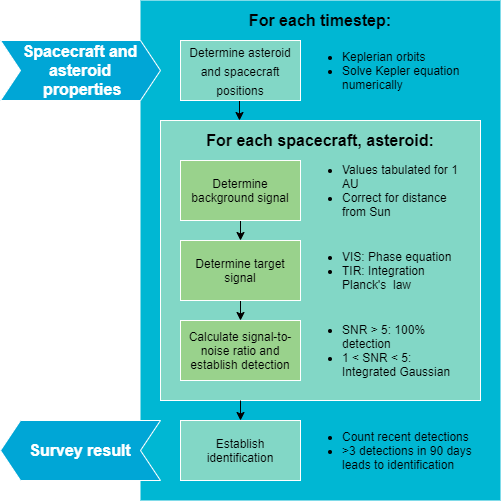
\includegraphics[width=0.7\textwidth]{img/simulation_overview.png}
 \caption{Overview of the simulation architecture and main loops.}
 \label{fig:simulation_overview}
\end{figure}

Currently, no model is publicly available for modelling multi-spacecraft surveys. Therefore, a simulation will be developed. During and after development, the model is also extensively verified and validated. The process for this is described in REF??. Other research (e.g. \cite{Flyeye}, \cite{2017NEOSDT}) has demonstrated the potential for explicitly modelling out the entire survey as it would be conducted by the actual system. This consists of first generating a representative population of asteroids (described in \autoref{sec:modelling_population}), then, at each timestep, calculating the background and target signal (\autoref{sec:modelling_background} and \autoref{sec:modelling_target}, respectively). Knowing these signals, the signal-to-noise ratios can then be determined after estimation of some of the detector properties (\autoref{sec:modelling_hardware_SNR}). The frequency and location of the observations is determined by the search strategy, and resulting cadence (detailed in \autoref{sec:modelling_cadence}) and lastly through repeat observations, it can be determined whether the system is capable of identifying a target (\autoref{sec:modelling_identification}).\\


The architecture of the simulation is shown in \autoref{fig:simulation_overview}. On the top left, the main input parameters to the model are displayed. These are primarily the spacecraft and asteroid properties. Both of these consist of a full set of Keplerian orbital elements per spacecraft or asteroid. The asteroid properties furthermore include the albedo, size, and absolute magnitude of each asteroid; the spacecraft properties include which type of payload the spacecraft is carrying. \\

The simulation consists of a nested loop. Firstly, at the start of each timestep (the time between the timesteps is determined by the survey cadence), the positions of all asteroids and spacecraft are determined by propagation of their orbital elements. Then, in the inside loop, each spacecraft is checked against each asteroid to see if it can detect said asteroid. This is done through calculation of the signal-to-noise ratio (SNR). Lastly, as it is known which asteroids got succesfully detected by which spacecraft, it can be determined if asteroids have been identified. Then, at the end of the simulation, the result is a list of the asteroid population in addition to whether they have been detected, and if so, when. Of course, this data can be further processed.

\section{Population of Asteroids}
\label{sec:modelling_population}
The first component of the simulation is the asteroid population model. This population was already briefly described in \autoref{sec:introduction_NEA}. In this section, more details on the generation of the population and the process of determining the positions of the NEA's, are given. As already mentioned in \autoref{sec:introduction_NEA}, the most comprehensive debiased population model is the one by \cite{PopulationGranvik}. This population model was generated by propagating an intiial population of NEA's based on several known interactions (e.g. gravitational interaction with the planets), and then comparing the resulting population to the results of the NEOWISE mission. Essentially, the problem then reduces to the question: ``What initial population would result in the results that are observed in the NEOWISE mission?''. Then, the initial population model can be fitted to the results of the NEOWISE mission, and an accurate population model is obtained. \\

Of course, this results in a full population of NEA's; whereas a population of \textit{unidentified} NEA's is required for this work. Therefore, a correction to the population was made based on the work of \cite{PopulationHarris}. To do this, the population as given by \cite{PopulationGranvik} was separated, based on absolute magnitude, into bins of width 0.5. Then, it was assumed that the detection of NEAs is roughly uniform over the orbital parameters. The completeness statistics of \cite{PopulationHarris} can then be used to discard a part of the population as \textit{identified}. For example, given 10000 asteroids in the bin width XXYYZZ, where 70\% is considered identified at this time, 7000 asteroids are selected at random and discarded. Of course, the assumption of uniformity in the detection of NEA's is false: highly eccentric NEA's, NEA's that are very dark, or NEA's with a high semi-major axis are more likely to be undetected. However, no data is available on this matter, and therefore no better alternative was deemed to be available. As all simulations will be affected equally, the error is judged to be sufficiently small for practical purposes.

\section{Background Signal}
\label{sec:modelling_background}

BESPREKEN BIJ IMPLEMENTATION: Hoe worden achtergrondsterren weggehaald?

Before considering the existing knowledge on modelling asteroid signals, first the background in which these targets has to be observed is discussed. In this section, the current relevant body of knowledge on modelling this background signal will be listed. The background signal will be split into two components. Firstly, the background light originating from the Sun. This manifests most dramatically in the form of direct Sunlight. However, also reflections off of interplantary dust are important. This reflection manifests in the phenomena of zodiacal light and gegenschein. The second component of the background signal, is the light from outside the Solar system. This light originates from other stars and manifests mainly as a diffuse background of starlight. In addition, a very large concentration of this starlight is found around the galactic plane. \\

The reason for separating the background signal into these two components is straightforward: in a reference frame fixed among the stars, the background signal from outside the Solar system is practically unchanging as the spacecraft moves around the Sun; the parallax of moving a few AU is negligible on galactic scales. In constrast, the contribution of light from our Sun is directly dependent on the position of the spacecraft with regards to the Sun. In the following sections, two primary reference frames are used: a heliocentric ecliptic reference frame (A right-handed reference frame whose principal plane is the ecliptic plane, origin at the center of the Sun, and the positive X-direction towards the vernal equinox), and a galactic reference frame (A right-handed reference frame whose principal plane is the plane of the Milky Way, origin at the center of the Sun, and positive X-direction towards the galactic core). The transformations between eclpitic longitude and latitude $(l_e, b_e)$ and galactic longitude and latitude $(l_g, b_g)$ are as follows:

\begin{align}
 b_g &= \sin ^{-1} (\sin b_e * \sin B_{NGP}) - \cos b_e \sin b_{NGP} \sin (l_e - l_{NGP} \\
 \sin l_g' &= \frac{\sin b_e \cos b_{NGP} + \cos b_e \sin b_{NGP} \sin (l_e - l_{NGP})}{\cos b_g} \\
 \cos l_g' &= \frac{\cos (l_e - l_{NGP}) \cos b_e}{\cos b_g} \\
 l_g &= \begin{cases}
        \sin ^{-1} (\sin l_g') + l_{GC}; & \cos l_g' \geq 0 \\
        \pi - \sin^{-1} (\sin l_g') + l_{GC}; & \cos l_g' < 0, \sin l_g' > 0 \\
        - \pi - \sin^{-1} (\sin l_g') + l_{GC}; & \cos l_g' < 0, \sin l_g' \leq 0
       \end{cases}
\end{align}

With $b_{NGP}$ the latitude of the North Galactic Pole, approximately equal to $29.81^\circ$ or $0.5203 \mathrm{rad}$; ascending node of the Galaxy $l_{NGP}$, approximately $270.02^\circ$, $4.712 \mathrm{rad}$; and longitude of the galactic core $l_{GC}$, approximately $6.38^\circ$, or $0.1114 \mathrm{rad}$. Finally, a transformation is required to express the ecliptic coordinates in a frame which is relative to the Sun, as the Sun-based contribution will be expressed relative to the Sun. This is however simply a subtraction of the latitude $l_e^\odot$ and longitude $b_e^\odot$ of the Sun in the ecliptic frame, from the latitude and longitude of the target in the eclpitic frame:
\begin{align}
 l_h &= l_e - l_e^\odot \\
 b_h &= b_e - b_e^\odot
\end{align}

With the reference frames defined, the individual components can be discussed. Firstly, the contribution of the Sun will be discussed, and then the background starlight for both thermal infrared and visual light.

\subsection{Solar contribution}
Modelling of the thermal infrared background radiation as a result of the light from the Sun is described by \cite{IRDust}, based on observations of the COBE mission. This model focusses on a modelling of the thermal state of interplanetary dust, and the resulting thermal infrared emission observed. Thus, the signal is not comprised of light originating at the Sun - but rather on the radiation from bodies heated by that light. The authors state that the albedo of particles at the relevant wavelengths is very close to zero, and therefore scattered Sunlight need not be considered; only the emissions of the particles. Thus, the zodiacal flux $Z(l, b)$ can be expresssed as an integral over the line of sight of the sensor of the various contributions (which will be discussed in  more detail below):
\begin{equation}
 Z(l, b) = \Sigma_c = \int _{\lambda_0} ^{\lambda_1} \int _S n_{c}(X, Y, Z)  E_{c}(\lambda) B(\lambda, T) ds d\lambda
 \label{eq:irdustflux}
\end{equation}
With $n_c$ being the density of the dust due to a contribution $c$, $B$ is the blackbody emission given by Planck's law and $E_c$ is a wavelength-specific emission correction factor. The temperature of the dust grains is assumed to follow a power law function of distance from the Sun $R$:
\begin{equation}
 T(R) = T_0R^{-0.467}
\end{equation}
Temperature $T_0$ at 1 AU is set to $286 \mathrm{K}$, and the emissivity modifications at the $4.9 \mu\mathrm{m}$ and $12 \mu\mathrm{m}$ thermal infrared wavelength are $0.997$ and $0.958$, respectively. Then, based on observations of the COBE mission, the authors construct a parametric model, based on three contributions. The first contribution is a ``donut-shaped'' dust cloud centered on the Sun, and inclined $2.03^\circ$ with respect to the ecliptic. This is the largest contributor to the density of interplanetary dust. Two more contributions which are modelled are a set of three dust bands, inclined at $0.56^\circ$, $1.2^\circ$ and $0.8^\circ$. Lastly, a circumsolar ring is modelled along the orbit of the Earth, which has a higher concentration around $10^\circ$ behind Earth in its orbit, as dust trails the planet due to its gravity. \footnote{For conciseness, the exact model will not be described here in detail; interested readers can refer to \cite{IRDust}.} An illustration of the contours of the components is seen in \autoref{fig:irdustcontributions}.\\

\begin{figure}[htbp]
 \centering
 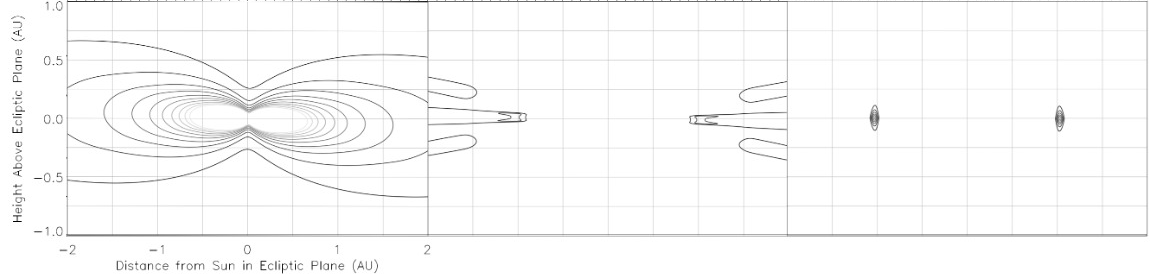
\includegraphics[width=1.0\textwidth]{img/ir_dust_components.png}
 \caption{Isodensity contours of the interplanetary dust model, shown at a plane perpendicular to the ecliptic. F.l.t.r.: the dust cloud, dust bands, and the circumsolar ring. Units of the contours are $10^{-7} \mathrm{AU}^{-1}$ for the dust cloud, and $0.125\cdot10^{-7} \mathrm{AU}^{-1}$ for the bands and ring.}
 \label{fig:irdustcontributions}
\end{figure}

The combined density model is shown in \autoref{fig:irdustcombined}. As can be seen, the dust cloud is the largest contributor to the density of the dust cloud. With the density and temperature components known, the infrared background due to the interplanetary dust can be modelled. The only factor that needs to be added to this is the direct thermal radiation from the Sun, which can be obtained directly from Planck's law. \\

\begin{figure}[htbp]
 \centering
 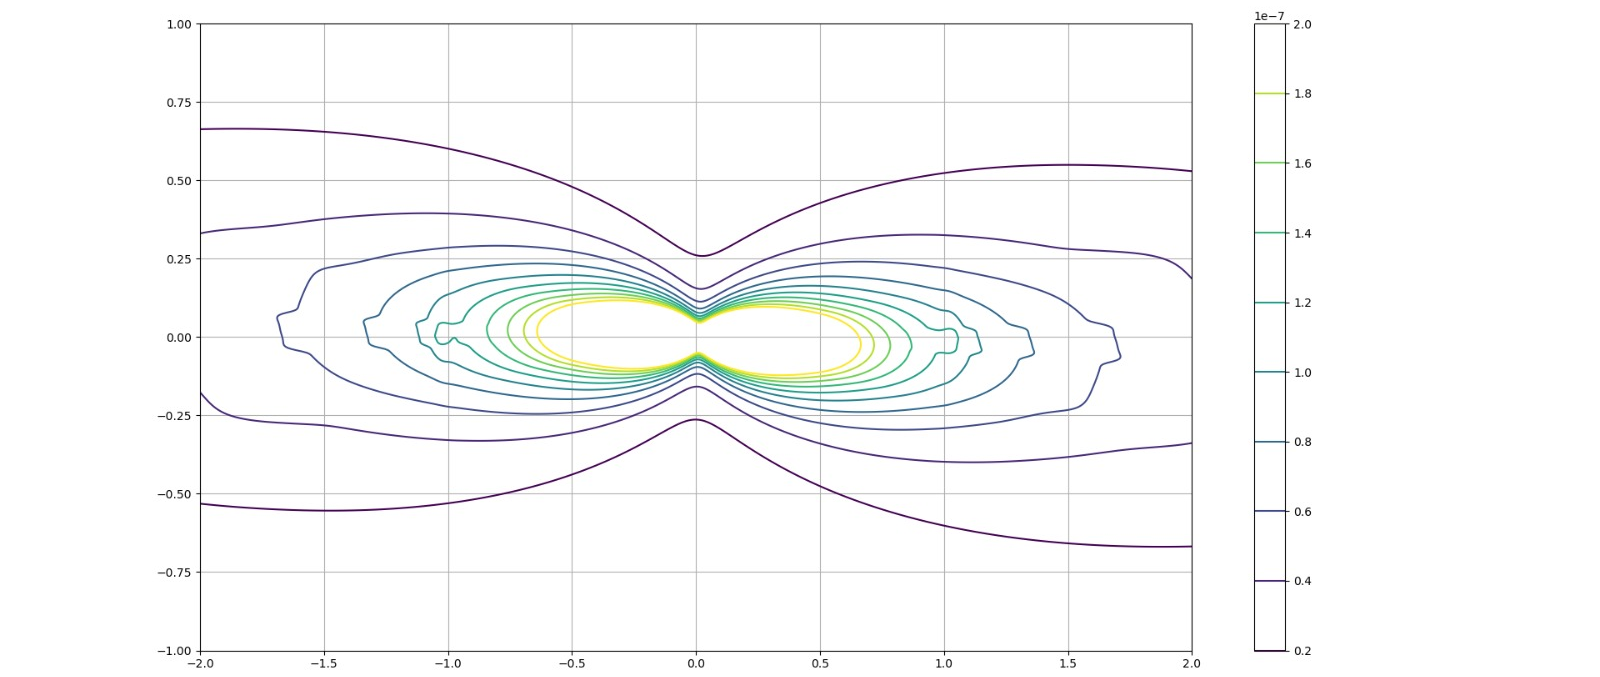
\includegraphics[width=0.9\textwidth]{img/ir_dust_combined.png}
 \caption{Combined isodensity contour of the interplanetary dust in a plane perpendicular to the ecliptic. TO DO: 3D PLOT}
 \label{fig:irdustcombined}
\end{figure}

Combining all these components leads to the full contribution as a result of Solar radiation and interplanetary dust. An illustration of the signal can be seen in \autoref{fig:solartirbackground}. The contribution from the Sun, and the hot dust near the Sun, is the most important source. However, there is still a sizeable flux originating in the interplanetary dust throughout the Solar system.\\

\begin{figure}[htbp]
 \centering
 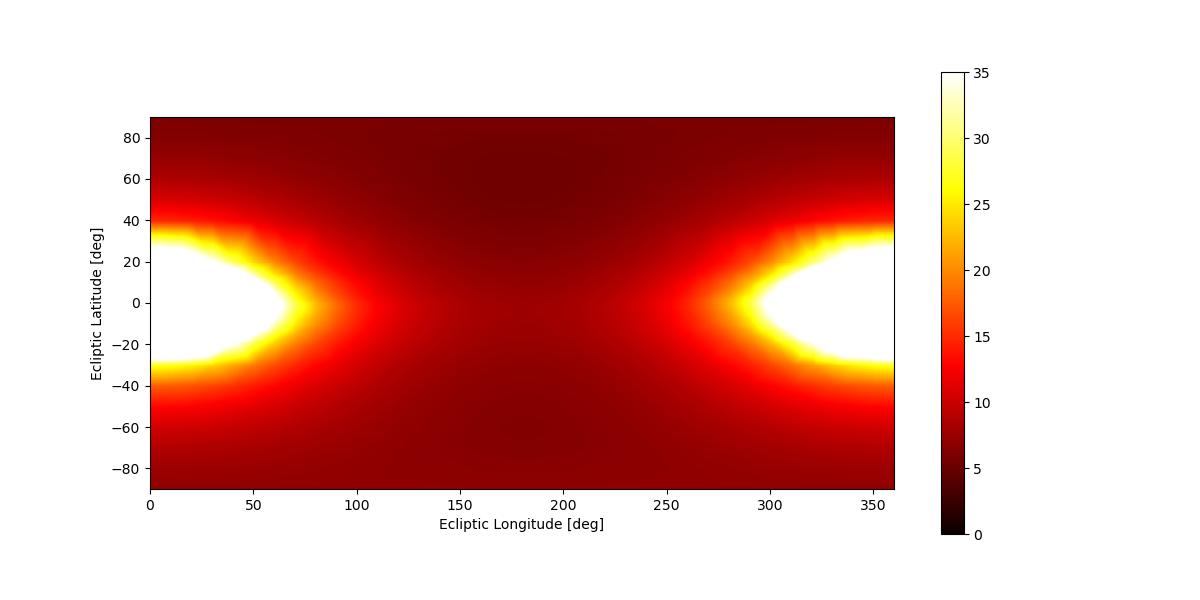
\includegraphics[width=1.0\textwidth]{img/background_tir_zodiac.png}
 \caption{Contribution of light from the Sun to the background signal in thermal infrared, in ecliptic coordinates, as seen from a spacecraft located at (-1, 0, 0) AU. Units are Megajansky per steradian, $1 \mathrm{MJy}{sr}^{-1} = 10^{-21} \mathrm{W}\mathrm{m}^{-2}\mathrm{Hz}^{-1}\mathrm{Sr}^{-1}$, and the scale is clipped at 35 $\mathrm{MJy}{sr}^{-1}$ for clarity.}
 \label{fig:solartirbackground}
\end{figure}

On the other hand, the background signal in the visual spectrum is more readily available. As it can be quickly and repeatedly measured from the surface of the Earth, early measurements of this signal exist. The components of the visual light background signal are tabulated by \cite{LightOfTheNightSky}, using data obtained from measurements. The resulting contribution from the Sun and Sunlight reflected off of interplanetary dust can be seen in \autoref{fig:solarvisbackground}. Next to the obvious contribution of the Sun and zodiacal light, the phenomenon of gegenschein can be observed in the middle of the plot. Although this is the points where target asteroids are brightests, it is also a point of increased background flux. The values as tabulated by \cite{LightOfTheNightSky} are only valid at a distance from the Sun of $1 \mathrm{AU}$. \cite{SkyBrightness} offer a correction factor for changing heliocentric position of the observer as follows:
\begin{equation}
 F(R) = F_{1\mathrm{AU}}R^{-2.3}
\end{equation}
This correction factor accounts for both the approximate decrease in interplanetary dust density when moving away from the Sun, as well as the decrease in solar flux. With these components, the Sun-dependent portion of the background signal is fully available for modelling. \\

\begin{figure}[htbp]
 \centering
 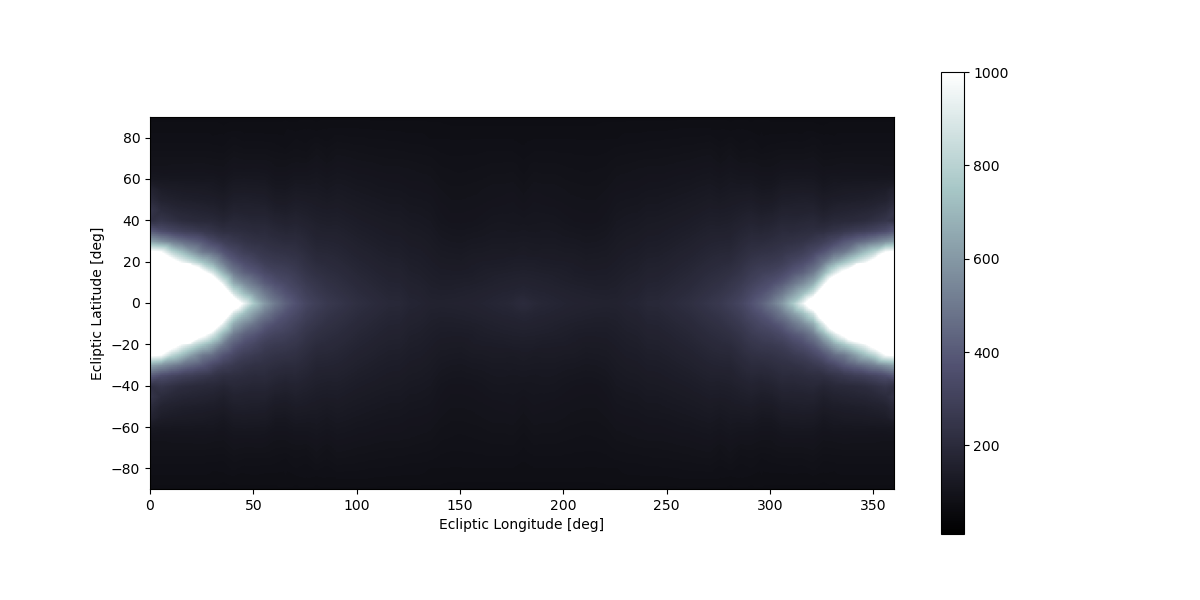
\includegraphics[width=1.0\textwidth]{img/background_vis_zodiac.png}
 \caption{Contribution of light form the Sun to the background signal in the visual spectrum, in ecliptic coordinates, as seen from a spacecraft located at (-1, 0, 0) AU. Units are $S10_\odot$ or solar-type stars of 10th magnitude per square degree. $1S10_\odot = 9.00\mathrm{W}\mathrm{m}^{-2}\mathrm{Sr}^{-1}$. The scale is clipped at $1000 S10_\odot$ for clarity.}
 \label{fig:solarvisbackground}
\end{figure}


\subsection{Milky Way and Diffuse Starlight}



\begin{figure}[htbp]
 \centering
 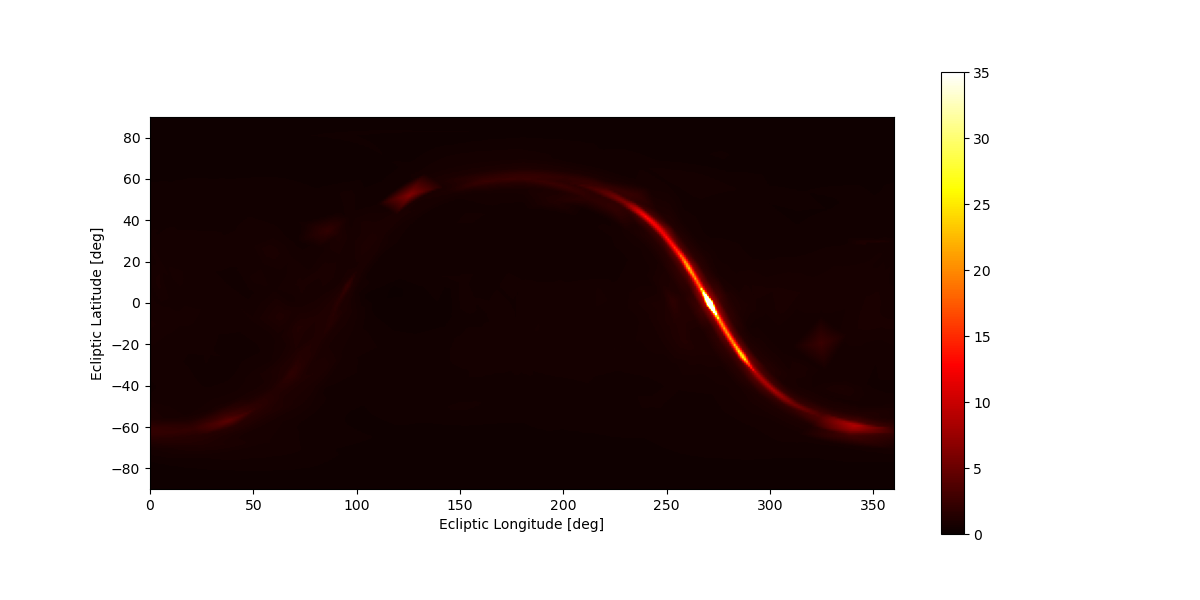
\includegraphics[width=1.0\textwidth]{img/background_tir_stars.png}
 \caption{Contribution of light from the Milky Way and diffuse starlight to the background signal in thermal infrared, in ecliptic coordinates. Units are Megajansky per steradian, $1 \mathrm{MJy}{sr}^{-1} = 10^{-21} \mathrm{W}\mathrm{m}^{-2}\mathrm{Hz}^{-1}\mathrm{Sr}^{-1}$, and the scale is clipped at 35 $\mathrm{MJy}{sr}^{-1}$ for clarity.}
 \label{fig:starstirbackground}
\end{figure}




\begin{figure}[htbp]
 \centering
 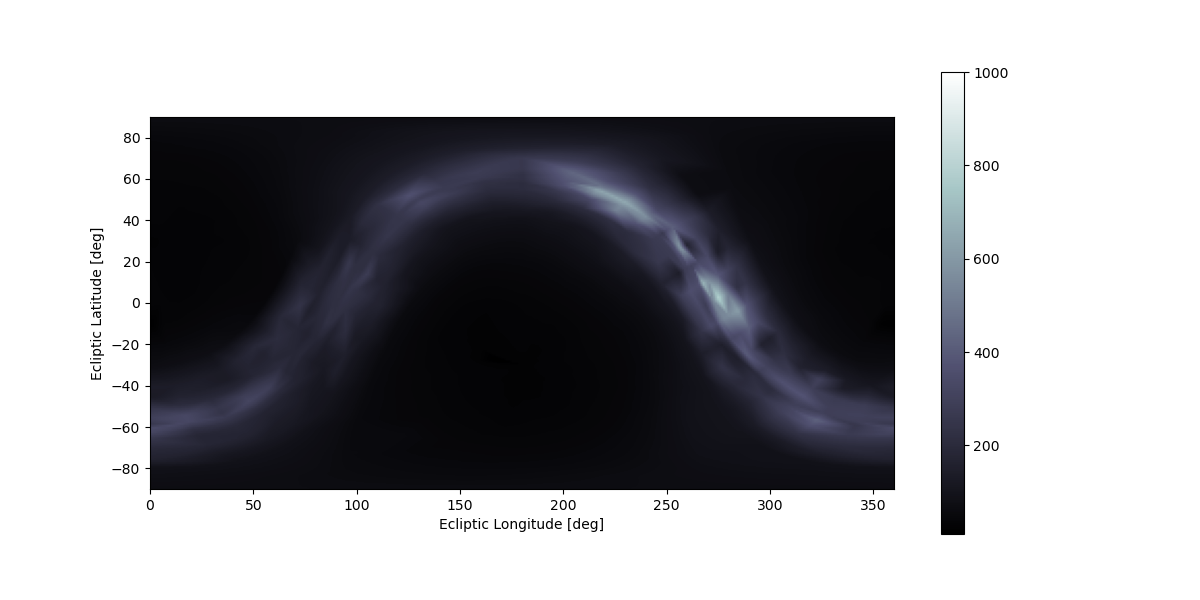
\includegraphics[width=1.0\textwidth]{img/background_vis_stars.png}
 \caption{Contribution of light form the Milky Way and diffuse starlight to the background signal in the visual spectrum, in ecliptic coordinates. Units are $S10_\odot$ or solar-type stars of 10th magnitude per square degree. $1S10_\odot = 9.00\mathrm{W}\mathrm{m}^{-2}\mathrm{Sr}^{-1}$. The scale is clipped at $1000 S10_\odot$ for clarity.}
 \label{fig:starsvisbackground}
\end{figure}


\section{Target Signal}
\label{sec:modelling_target}

\section{Hardware Properties and Signal-to-Noise Ratio}
\label{sec:modelling_hardware_SNR}

\section{Search Strategy and Cadence}
\label{sec:modelling_cadence}

\section{Detection and Identification}
\label{sec:modelling_identification}
